% Editorial bootstrap from the immutable source revision.
% This file is canonical and may be edited independently.

\part{Dyadic Self-Sampling and Alias Superconvergence}


% Source fragment: Inverse and sampling frontiers; prefix is.
\section{Normalization and established structure}
\label{is:p3:sec:background}

\subsection{The up-law, Fabius function, and Fourier convention}

Let $u=\RvachevUp$ be Rvachev's even nonnegative $C^\infty$ function supported on $[-1,1]$, normalized by
\[
 \int_{-1}^{1}u(x)\Differential x=1,
 \qquad u(0)=1.
\]
We use
\begin{equation}
 \FourierTwoPi{f}(\xi)=\int_{\RealNumbers}f(x)\EulerE^{-2\pi\iu x\xi}\Differential x,
 \qquad
 \PhiCyc(\xi)=\FourierTwoPi{u}(\xi)
 =\prod_{j=0}^{\infty}\SincPi\!\left(\frac{\xi}{2^j}\right),
 \label{is:p3:eq:Phi-product}
\end{equation}
where
\[
 \SincPi z=\begin{cases}\dfrac{\sin(\pi z)}{\pi z},&z\ne0,\\[0.4em]1,&z=0.\end{cases}
\]
The product is entire.  If $m\in\IntegerNumbers\setminus\{0\}$, then
\begin{equation}
 \OrderOperator_{\xi=m}\PhiCyc=1+\nu_2(m).
 \label{is:p3:eq:integer-multiplicity}
\end{equation}
Indeed, the factors indexed by $0\le j\le\nu_2(m)$ vanish simply and all later factors are nonzero.

This foundation is now formal rather than merely inherited from the human
corpus.  The standalone product is entire by
\path{Fabius.rvachevFourierProduct_differentiable}; for every nonzero
integer \(m\), Lean proves
\[
 \OrderOperator_{\xi=m}\PhiCyc=1+\nu_2(|m|)
\]
as \path{Fabius.analyticOrderAt_rvachevFourierProduct_int}, together with
all lower derivative vanishings and the exact nonzero leading derivative
in \path{IntegerZeroAnalyticOrder.lean}.

The standard Fabius distribution function $F:[0,1]\to[0,1]$ is related to $u$ by
\begin{equation}
 u(x)=F(1-\AbsoluteValue{x})\quad (\AbsoluteValue{x}\le1),
 \qquad
 F(t)=u(t-1)\quad(0\le t\le1).
 \label{is:p3:eq:F-up-relation}
\end{equation}
If $Y$ has density $u$, then
\begin{equation}
 \Probability(Y\le x)=F\!\left(\frac{x+1}{2}\right),
 \qquad -1\le x\le1.
 \label{is:p3:eq:centered-CDF}
\end{equation}
Thus the centered quantile is
\begin{equation}
 q(t)=2F^{-1}(t)-1.
 \label{is:p3:eq:centered-quantile}
\end{equation}

\subsection{Moments, moment generating function, and cumulants}

Write
\begin{equation}
 \mu_n=\int_{-1}^{1}x^n u(x)\Differential x,
 \qquad c_n=\mu_{2n}.
 \label{is:p3:eq:moments}
\end{equation}
Odd moments vanish.  The even moments are rational and satisfy
\begin{equation}
 (2n+1)(2^{2n}-1)c_n
 =\sum_{k=0}^{n-1}\binom{2n+1}{2k}c_k,
 \qquad c_0=1.
 \label{is:p3:eq:moment-recurrence}
\end{equation}
The moment generating function is
\begin{align}
 M(z)
 &=\int_{-1}^{1}\EulerE^{zx}u(x)\Differential x
 =\PhiCyc\!\left(\frac{\iu z}{2\pi}\right)\notag\\
 &=\prod_{j=0}^{\infty}
 \frac{\sinh(z/2^{j+1})}{z/2^{j+1}}.
 \label{is:p3:eq:mgf-product}
\end{align}
Its logarithm has even cumulants
\begin{equation}
 \log M(z)=\sum_{r=1}^{\infty}\kappa_{2r}\frac{z^{2r}}{(2r)!},
 \qquad
 \boxed{\displaystyle
 \kappa_{2r}=\frac{B_{2r}}{2r}\,
 \frac{2^{2r}}{2^{2r}-1}},
 \label{is:p3:eq:cumulants}
\end{equation}
where $B_n$ are Bernoulli numbers with $B_2=1/6$.  Consequently
\begin{equation}
 \mu_n=Y_n(0,\kappa_2,0,\kappa_4,\ldots,\kappa_n),
 \label{is:p3:eq:moment-Bell}
\end{equation}
with $Y_n$ the complete exponential Bell polynomial.

\subsection{Exact dyadic arithmetic}

For $0\le a\le2^n$, the corpus gives the finite moment--Thue--Morse formula
\begin{equation}
 F\!\left(\frac a{2^n}\right)
 =\frac{2^{-n(n+1)/2}}{n!}
 \sum_{h=0}^{a-1}\eps_h
 \sum_{k=0}^{\Floor{n/2}}
 \binom n{2k}(2a-2h-1)^{n-2k}c_k,
 \label{is:p3:eq:finite-F-moment}
\end{equation}
where $\eps_h=(-1)^{\BinaryDigitSum(h)}$.  In particular every dyadic sample of $F$ and $u$ is rational.  A second exact formula, recalled in \cref{is:p3:sec:qbinomial}, expresses the same value through Gaussian binomial coefficients at $q=1/2$ and finite signed Thue--Morse power sums.

\section{The shifted dyadic self-sampling theorem}
\label{is:p3:sec:self-sampling}

\subsection{Definition of the rules}

For $N\ge0$, $h_N=2^{-N}$, and phase $\theta\in\RealNumbers$, define
\begin{equation}
 Q_{N,\theta}[f]
 :=h_N\sum_{k\in\IntegerNumbers}
 f\bigl(h_N(k+\theta)\bigr)
 u\bigl(h_N(k+\theta)\bigr).
 \label{is:p3:eq:Q-def}
\end{equation}
Because $u$ is supported on $[-1,1]$, this is a finite sum.  The nodes are equally spaced, but the weights
\begin{equation}
 w_{N,\theta,k}=h_Nu\bigl(h_N(k+\theta)\bigr)
 \label{is:p3:eq:self-weights}
\end{equation}
are samples of the target density itself.  They are nonnegative and strictly positive at every interior node.

\begin{theorem}[Shifted self-sampling quadrature]
\label{is:p3:thm:self-sampling}
For every $N\ge0$, every $\theta\in\RealNumbers$, and every polynomial $p$ with $\deg p\le N$,
\begin{equation}
 \boxed{\displaystyle
 \int_{-1}^{1}p(x)u(x)\Differential x
 =2^{-N}\sum_{k\in\IntegerNumbers}
 p\!\left(\frac{k+\theta}{2^N}\right)
 u\!\left(\frac{k+\theta}{2^N}\right).}
 \label{is:p3:eq:self-sampling-main}
\end{equation}
In particular, $\sum_k w_{N,\theta,k}=1$, so the rule is a positive probability measure matching the first $N$ moments of $u$.
\end{theorem}

\begin{proof}
Let $0\le r\le N$ and set $f_r(x)=x^ru(x)$.  Since $u\in C_c^\infty(\RealNumbers)$, Poisson summation applies without regularization.  For the shifted lattice,
\begin{equation}
 h_N\sum_{k\in\IntegerNumbers}f_r\bigl(h_N(k+\theta)\bigr)
 =\sum_{\ell\in\IntegerNumbers}\EulerE^{2\pi\iu\ell\theta}
 \FourierTwoPi{f_r}(2^N\ell).
 \label{is:p3:eq:shifted-Poisson}
\end{equation}
Differentiating \eqref{is:p3:eq:Phi-product},
\begin{equation}
 \FourierTwoPi{f_r}(\xi)=\frac{\PhiCyc^{(r)}(\xi)}{(-2\pi\iu)^r}.
 \label{is:p3:eq:monomial-transform}
\end{equation}
The term $\ell=0$ is $\mu_r$.  If $\ell\ne0$, then \eqref{is:p3:eq:integer-multiplicity} gives
\[
 \OrderOperator_{\xi=2^N\ell}\PhiCyc
 =N+1+\nu_2(\ell)>r,
\]
so $\PhiCyc^{(r)}(2^N\ell)=0$.  Thus every nonzero alias vanishes, proving the identity for monomials and hence for all polynomials of degree at most $N$.
\end{proof}

\begin{remark}[A dyadic Strang--Fix phenomenon]
Classical Strang--Fix conditions turn zeros of a generator's Fourier transform at the dual lattice into polynomial reproduction by shifts.  Here the generator also supplies the quadrature weights.  The result is therefore a self-weighted, positive, shifted Strang--Fix rule rather than a cardinal interpolation formula.  The exact order is read directly from the $2$-adic multiplicities of the sinc product.
\end{remark}

\subsection{Rationality and denominator control}

\begin{corollary}[Positive rational rules]
\label{is:p3:cor:rational-rules}
If $\theta=a/2^s$ is dyadic, every node and every weight in \eqref{is:p3:eq:self-sampling-main} is rational.  More explicitly, with
\[
 D=N+s,
 \qquad n_k=2^sk+a,
 \qquad b_k=2^D-\AbsoluteValue{n_k},
\]
one has, whenever $\AbsoluteValue{n_k}<2^D$,
\begin{equation}
 x_k=\frac{n_k}{2^D},
 \qquad
 w_k=2^{-N}F\!\left(\frac{b_k}{2^D}\right)\in\RationalNumbers_{>0}.
 \label{is:p3:eq:rational-weights}
\end{equation}
A common denominator for all such weights is obtained by multiplying the repository's level-$D$ dyadic denominator bound by $2^N$.
\end{corollary}

\begin{proof}
Use \eqref{is:p3:eq:F-up-relation} at the dyadic node $x_k$.  The denominator assertion follows from the established bound
\[
 D!\,2^{\binom{D+1}{2}}(2\Floor{D/2}+1)!!
 \prod_{j=1}^{\Floor{D/2}}(2^{2j}-1)\,u(n/2^D)\in\NaturalNumbers
\]
for $\AbsoluteValue n<2^D$.
\end{proof}

\subsection{Finite moment identities in Fabius values}

For the centered phase $\theta=0$, symmetry yields particularly transparent formulas.  For $r\ge1$ with $2r\le N$,
\begin{equation}
 \boxed{\displaystyle
 c_r=2^{1-N-2rN}
 \sum_{j=1}^{2^N-1}(2^N-j)^{2r}
 F\!\left(\frac j{2^N}\right).}
 \label{is:p3:eq:centered-moment-F}
\end{equation}
For $r=0$, normalization reads
\begin{equation}
 1=2^{-N}\left(1+2\sum_{j=1}^{2^N-1}F\!\left(\frac j{2^N}\right)\right).
 \label{is:p3:eq:centered-normalization-F}
\end{equation}
These are positive finite identities: the moment on the left is reconstructed from values of the Fabius function with no alternating coefficients.

\begin{proof}
Apply \cref{is:p3:thm:self-sampling} to $p(x)=x^{2r}$.  Pair the nodes $\pm k/2^N$, use $u(k/2^N)=F(1-k/2^N)$, and then put $j=2^N-k$.
\end{proof}

\begin{resultbox}[First frontier bridge]
The exact dyadic values in the corpus were previously used primarily as point evaluations, denominator data, or inputs to signed extrapolation.  Equations \eqref{is:p3:eq:self-sampling-main}--\eqref{is:p3:eq:centered-moment-F} instead organize them as a hierarchy of positive moment designs.  Fourier zero multiplicities, dyadic rationality, and probability positivity become three faces of one formula.
\end{resultbox}

\section{The master alias function and the
\texorpdfstring{$2$}{2}-adic error filtration}
\label{is:p3:sec:alias}

\subsection{An entire generating function for all moment defects}

Define
\begin{equation}
 G_{N,\theta}(z)
 :=Q_{N,\theta}[\EulerE^{zx}]-M(z).
 \label{is:p3:eq:G-def}
\end{equation}
The coefficient of $z^r/r!$ is exactly the $r$th moment defect
\begin{equation}
 E_{N,r}(\theta)
 :=Q_{N,\theta}[x^r]-\mu_r.
 \label{is:p3:eq:ENr-def}
\end{equation}

\begin{theorem}[Master shifted-alias identity]
\label{is:p3:thm:master-alias}
For every $N\ge0$, $\theta\in\RealNumbers$, and $z\in\ComplexNumbers$,
\begin{equation}
 \boxed{\displaystyle
 G_{N,\theta}(z)
 =\sum_{\ell\in\IntegerNumbers\setminus\{0\}}
 \EulerE^{2\pi\iu\ell\theta}
 \PhiCyc\!\left(2^N\ell+\frac{\iu z}{2\pi}\right).}
 \label{is:p3:eq:master-alias}
\end{equation}
The series is locally normally convergent.  Moreover $G_{N,\theta}$ has a zero of order at least $N+1$ at $z=0$.
\end{theorem}

\begin{proof}
Apply shifted Poisson summation to $f_z(x)=\EulerE^{zx}u(x)$.  Its Fourier transform is
\[
 \FourierTwoPi{f_z}(\xi)
 =\PhiCyc\!\left(\xi+\frac{\iu z}{2\pi}\right).
\]
The zero-frequency term is $M(z)$, giving \eqref{is:p3:eq:master-alias}.  Compact support and smoothness imply the local normal convergence needed to differentiate termwise.  At $z=0$, the summand indexed by $\ell\ne0$ has order
$N+1+\nu_2(\ell)$, so the full sum begins at order $N+1$.
\end{proof}

\begin{corollary}[Valuation filtration of polynomial errors]
\label{is:p3:cor:valuation-filtration}
For $r>N$,
\begin{equation}
 E_{N,r}(\theta)
 =\frac1{(-2\pi\iu)^r}
 \sum_{a=0}^{r-N-1}
 \sum_{\substack{q\in\IntegerNumbers\setminus\{0\}\\q\ \mathrm{odd}}}
 \EulerE^{2\pi\iu 2^aq\theta}
 \PhiCyc^{(r)}(2^{N+a}q).
 \label{is:p3:eq:valuation-filtration}
\end{equation}
Thus the excess degree $r-N$ exposes exactly the first $r-N$ layers of the $2$-adic alias tree.
\end{corollary}

\begin{proof}
In the coefficient formula obtained from \eqref{is:p3:eq:master-alias}, an alias $\ell$ can contribute only if
$N+1+\nu_2(\ell)\le r$.  Write $\ell=2^aq$ with $q$ odd.
\end{proof}

\begin{remark}
The first failure, $r=N+1$, sees only odd aliases.  The next failure, $r=N+2$, sees odd aliases and twice-odd aliases.  Higher defects are therefore not arbitrary: they are a triangular sequence of $2$-adic spectral layers.  This observation will be the basis of the next-defect conjectures in \cref{is:p3:sec:frontier}.
\end{remark}

\subsection{An exact local factorization at every integer zero}

The integer zero jets can be organized in a form that makes Bell polynomials appear automatically.

\begin{proposition}[Exact local factorization]
\label{is:p3:prop:local-factorization}
Let $m=2^{d-1}q\ne0$, where $q$ is odd and $d=1+\nu_2(m)$.  Then, for $w$ near $0$,
\begin{equation}
 \boxed{\displaystyle
 \PhiCyc(m+w)
 =-\left(\frac{w}{m+w}\right)^d
 \left(\prod_{j=0}^{d-1}\SincPi\!\left(\frac{w}{2^j}\right)\right)
 \PhiCyc\!\left(\frac q2+\frac{w}{2^d}\right).}
 \label{is:p3:eq:local-factorization}
\end{equation}
In particular,
\begin{equation}
 \PhiCyc(m+w)=C_mw^d
 \exp\!\left(\sum_{j\ge1}\gamma_j(m)\frac{w^j}{j!}\right),
 \qquad
 C_m=-\frac{\PhiCyc(q/2)}{m^d},
 \label{is:p3:eq:local-Bell-form}
\end{equation}
where the logarithmic jet $\gamma_j(m)$ is explicit.
\end{proposition}

\begin{proof}
For $0\le j\le d-1$, $m/2^j$ is an integer and
\[
 \SincPi\!\left(\frac{m+w}{2^j}\right)
 =(-1)^{m/2^j}\frac{w}{m+w}
 \SincPi\!\left(\frac{w}{2^j}\right).
\]
The product of the signs is $-1$ because
\[
 \sum_{j=0}^{d-1}\frac m{2^j}=q(2^d-1)
\]
is odd.  The remaining tail is
\[
 \prod_{j=d}^{\infty}\SincPi\!\left(\frac{m+w}{2^j}\right)
 =\PhiCyc\!\left(\frac q2+\frac{w}{2^d}\right).
\]
This proves \eqref{is:p3:eq:local-factorization}; taking the analytic logarithm after removing $C_mw^d$ gives \eqref{is:p3:eq:local-Bell-form}.
\end{proof}

\begin{statusbox}[Lean status of the local factorization]
Equation \eqref{is:p3:eq:local-factorization} is now formal in a stronger total,
denominator-cleared form valid for every complex \(w\), including the
removable points.  The all-nonzero-integer statement is
\path{Fabius.rvachevFourierProduct_int_add_factorization}; its divided
germ form is
\path{Fabius.rvachevFourierProduct_int_add_eventuallyEq_pow_mul_cofactor}.
The cofactor is analytic and nonzero at the local origin, so Lean proves the exact order, every
lower-jet vanishing, and the leading identity
\eqref{is:p3:eq:first-zero-jet}.  More generally, if that cofactor is denoted by
\(U_m\) and \(d=1+\nu_2(|m|)\), Lean proves every higher jet as
\[
 \PhiCyc^{(d+r)}(m)=\binom{d+r}{d}d!\,U_m^{(r)}(0)
 \qquad(r\in\NaturalNumbers)
\]
in \path{Fabius.iteratedDeriv_rvachevFourierProduct_int_add_order}.
The generic engine in \path{LeadingJet.lean} is vector-valued and computes
every derivative index over an arbitrary nontrivially normed field.  The
explicit normalization in \eqref{is:p3:eq:local-Bell-form}, the logarithmic coefficients
\eqref{is:p3:eq:gamma1}--\eqref{is:p3:eq:gamma-general} and the Bell-polynomial formula
\eqref{is:p3:eq:Bell-zero-jets} for \(s>0\) remain human-readable frontier
results, not named Lean theorems.
\end{statusbox}

The first logarithmic coefficient is especially simple:
\begin{equation}
 \gamma_1(m)=-\frac d m
 +2^{-d}\frac{\PhiCyc'(q/2)}{\PhiCyc(q/2)}.
 \label{is:p3:eq:gamma1}
\end{equation}
For general $j$,
\begin{equation}
 \gamma_j(m)
 =d(-1)^j\frac{(j-1)!}{m^j}
 +\sum_{h=0}^{d-1}2^{-hj}\ell_j
 +2^{-dj}L_j(q/2),
 \label{is:p3:eq:gamma-general}
\end{equation}
where
\[
 \ell_j=\left.\frac{\Differential^j}{\Differential z^j}\log\SincPi z\right|_{z=0},
 \qquad
 L_j(t)=\frac{\Differential^j}{\Differential t^j}\log\PhiCyc(t).
\]
The universal local coefficients satisfy
\begin{equation}
 \ell_{2r}=-\frac{(2r)!}{r}\zeta(2r),
 \qquad \ell_{2r+1}=0,
 \label{is:p3:eq:sinc-log-jet}
\end{equation}
so Bernoulli numbers may be substituted through Euler's formula for $\zeta(2r)$.

\begin{corollary}[Bell-polynomial zero jets]
\label{is:p3:cor:Bell-zero-jets}
With the notation of \cref{is:p3:prop:local-factorization}, for every $s\ge0$,
\begin{equation}
 \boxed{\displaystyle
 \PhiCyc^{(d+s)}(m)
 =C_m\frac{(d+s)!}{s!}
 Y_s\bigl(\gamma_1(m),\ldots,\gamma_s(m)\bigr).}
 \label{is:p3:eq:Bell-zero-jets}
\end{equation}
Here $Y_0=1$.  Consequently every layer of \eqref{is:p3:eq:valuation-filtration} has a finite Bell-polynomial description in half-integer logarithmic derivatives, zeta values, and elementary $2$-adic data.
\end{corollary}

\begin{proof}
Use the defining exponential generating function
\[
 \exp\!\left(\sum_{j\ge1}x_j\frac{w^j}{j!}\right)
 =\sum_{s\ge0}Y_s(x_1,\ldots,x_s)\frac{w^s}{s!}
\]
in \eqref{is:p3:eq:local-Bell-form} and compare coefficients.
\end{proof}

\begin{resultbox}[Second frontier bridge]
The corpus already contains the integer zero multiplicities and several zero-jet formulas.  The new point here is their use as an \emph{error calculus}: the excess polynomial degree selects a finite set of $2$-adic alias layers, and every derivative on those layers is generated by a complete Bell polynomial.  Bernoulli/zeta data enter locally through $\log\SincPi$, while Thue--Morse data enter globally through the half-integer tail.
\end{resultbox}

\section{The first defect: half-integer spectrum and Thue--Morse signs}
\label{is:p3:sec:first-defect}

Put
\begin{equation}
 r=N+1,
 \qquad
 E_N(\theta):=E_{N,N+1}(\theta).
 \label{is:p3:eq:first-defect-def}
\end{equation}
Only odd aliases survive.

\begin{theorem}[Exact first-defect series]
\label{is:p3:thm:first-defect}
For every $N\ge0$ and $\theta\in\RealNumbers$,
\begin{equation}
 \boxed{\displaystyle
 E_N(\theta)
 =-\frac{r!}{(-2\pi\iu)^r2^{Nr}}
 \sum_{\substack{\ell\in\IntegerNumbers\setminus\{0\}\\\ell\ \mathrm{odd}}}
 \frac{\PhiCyc(\ell/2)}{\ell^r}
 \EulerE^{2\pi\iu\ell\theta}.}
 \label{is:p3:eq:first-defect-complex}
\end{equation}
Equivalently, if $r=2s$,
\begin{equation}
 E_N(\theta)
 =\frac{2(-1)^{s+1}r!}{(2\pi)^r2^{Nr}}
 \sum_{\substack{m\ge1\\m\ \mathrm{odd}}}
 \frac{\PhiCyc(m/2)}{m^r}\cos(2\pi m\theta),
 \label{is:p3:eq:first-defect-even}
\end{equation}
and if $r=2s+1$,
\begin{equation}
 E_N(\theta)
 =\frac{2(-1)^sr!}{(2\pi)^r2^{Nr}}
 \sum_{\substack{m\ge1\\m\ \mathrm{odd}}}
 \frac{\PhiCyc(m/2)}{m^r}\sin(2\pi m\theta).
 \label{is:p3:eq:first-defect-odd}
\end{equation}
\end{theorem}

\begin{proof}
For $m=2^N\ell$ with $\ell$ odd, \cref{is:p3:prop:local-factorization} with $d=r$ gives
\begin{equation}
 \PhiCyc^{(r)}(2^N\ell)
 =-\frac{r!\PhiCyc(\ell/2)}{(2^N\ell)^r}.
 \label{is:p3:eq:first-zero-jet}
\end{equation}
Insert this into \eqref{is:p3:eq:valuation-filtration}.  Pair positive and negative odd frequencies to obtain the real forms.
\end{proof}

\subsection{The spectral sign is exactly Thue--Morse}

\begin{proposition}[Half-integer sign law]
\label{is:p3:prop:half-integer-sign}
For $j\ge0$,
\begin{equation}
 \Sign\PhiCyc\!\left(\frac{2j+1}{2}\right)
 =(-1)^{\BinaryDigitSum(j)}=\eps_j.
 \label{is:p3:eq:half-integer-sign}
\end{equation}
Hence the first quadrature defect is a Thue--Morse-signed half-integer spectral Dirichlet series.
\end{proposition}

\begin{proof}
On the positive real axis, $\PhiCyc$ changes sign whenever an integer zero has odd multiplicity.  At the point $(2j+1)/2=j+1/2$, the total number of zero crossings, counted with multiplicity, is
\[
 \sum_{m=1}^{j}\bigl(1+\nu_2(m)\bigr)
 =j+\nu_2(j!)
 =2j-\BinaryDigitSum(j),
\]
where the last equality is Legendre's formula
$\nu_2(j!)=j-\BinaryDigitSum(j)$.  Its parity is therefore
$\BinaryDigitSum(j)$.  Since $\PhiCyc(1/2)>0$, the claimed sign follows.
\end{proof}

Writing
\begin{equation}
 a_j=\AbsoluteValue{\PhiCyc((2j+1)/2)},
 \label{is:p3:eq:half-amplitudes}
\end{equation}
we may rewrite the spectral coefficient as $\PhiCyc((2j+1)/2)=\eps_ja_j$.  Thus the signs are purely digital, while the amplitudes record the sinc-product decay.

\subsection{Symmetries}

\begin{corollary}[Phase symmetries]
\label{is:p3:cor:defect-symmetries}
The first defect is $1$-periodic and satisfies
\begin{equation}
 E_N(-\theta)=(-1)^rE_N(\theta),
 \qquad
 E_N(\theta+1/2)=-E_N(\theta).
 \label{is:p3:eq:defect-symmetries}
\end{equation}
\end{corollary}

\begin{proof}
The first identity follows from the sine/cosine parity.  The second follows because every frequency in \eqref{is:p3:eq:first-defect-complex} is odd.
\end{proof}

\section{A Bernoulli convolution formula for the first defect}
\label{is:p3:sec:bernoulli-kernel}

\subsection{The periodic up-kernel}

Define a $1$-periodic continuous function $\Kcal$ by
\begin{equation}
 \Kcal(t)=2u(2t)-1,
 \qquad -\frac12\le t\le\frac12,
 \label{is:p3:eq:K-kernel}
\end{equation}
with periodic extension.  Its mean is zero.  For $n\ne0$, its Fourier coefficient is
\begin{equation}
 \FourierSeriesCoefficient{\Kcal}{n}
 =\int_{-1/2}^{1/2}\Kcal(t)\EulerE^{-2\pi\iu nt}\Differential t
 =\PhiCyc(n/2).
 \label{is:p3:eq:K-Fourier}
\end{equation}
In particular the even nonzero coefficients vanish, and the odd coefficients carry the Thue--Morse signs of \cref{is:p3:prop:half-integer-sign}.

Let $\Bper_r(t)=B_r(\{t\})$ be the periodic Bernoulli polynomial, understood in the standard Fourier/distributional sense when $r=1$.  For $n\ne0$,
\begin{equation}
 \FourierSeriesCoefficient{\Bper_r}{n}=-\frac{r!}{(2\pi\iu n)^r}.
 \label{is:p3:eq:periodic-Bernoulli-Fourier}
\end{equation}

\begin{theorem}[Bernoulli--Rvachev error kernel]
\label{is:p3:thm:Bernoulli-convolution}
For $r=N+1$,
\begin{equation}
 \boxed{\displaystyle
 E_N(\theta)=(-1)^r2^{-Nr}
 (\Bper_r*\Kcal)(\theta),}
 \label{is:p3:eq:Bernoulli-convolution}
\end{equation}
where convolution is on $\RealNumbers/\IntegerNumbers$.
\end{theorem}

\begin{proof}
Multiply the nonzero Fourier coefficients in \eqref{is:p3:eq:K-Fourier} and \eqref{is:p3:eq:periodic-Bernoulli-Fourier}.  The resulting Fourier series is exactly \eqref{is:p3:eq:first-defect-complex}; the even frequencies vanish automatically.
\end{proof}

\begin{remark}
This formula is not an Euler--Maclaurin expansion with an unspecified remainder.  It is an exact identity.  The universal periodic Bernoulli kernel describes polynomial aliasing, while $\Kcal$ inserts the complete half-integer spectrum of the up-law.  It therefore provides a direct analytical bridge from Bernoulli polynomials to the Rvachev sinc product.
\end{remark}

\subsection{A rigorous first-harmonic bound}

\begin{lemma}[Finite product loss bound]
\label{is:p3:lem:finite-product-loss}
If $0\le a_j\le1$ for $0\le j\le J$, then
\begin{equation}
 \prod_{j=0}^{J}(1-a_j)\ge1-\sum_{j=0}^{J}a_j.
 \label{is:p3:eq:finite-product-loss}
\end{equation}
\end{lemma}

\begin{proof}
The assertion is equality for $J=0$.  If it holds through $J-1$, put
$S=\sum_{j=0}^{J-1}a_j$.  Multiplication by the nonnegative number
$1-a_J$ and the induction hypothesis give
\[
 \prod_{j=0}^{J}(1-a_j)
 \ge(1-S)(1-a_J)
 =1-S-a_J+Sa_J
 \ge1-S-a_J.
\]
This proves the induction step.
\end{proof}

\begin{lemma}[A uniform lower bound at the first half-integer]
\label{is:p3:lem:phi-half-lower}
\begin{equation}
 \PhiCyc(1/2)>1-\frac{\pi^2}{18}>\frac49.
 \label{is:p3:eq:phi-half-lower}
\end{equation}
\end{lemma}

\begin{proof}
For $0\le x\le1/2$, $\SincPi x\ge1-\pi^2x^2/6$.  Set
$a_j=(\pi^2/6)4^{-(j+1)}$.  All $a_j$ lie in $(0,1)$, and
\cref{is:p3:lem:finite-product-loss}, followed by passage to the limit, gives
\[
 \PhiCyc(1/2)\ge\prod_{j=0}^{\infty}(1-a_j).
\]
This product is strictly larger than $1-\sum_ja_j$.  Indeed, if
$S=\sum_{j=2}^{\infty}a_j$, another application of the finite product bound
to the tail and passage to the limit yield
\begin{align*}
 \prod_{j=0}^{\infty}(1-a_j)
 &\ge(1-a_0)(1-a_1)(1-S)\\
 &=1-a_0-a_1-S
   +a_0a_1+S(a_0+a_1-a_0a_1)\\
 &>1-a_0-a_1-S.
\end{align*}
Consequently
\[
 \PhiCyc(1/2)>1-\frac{\pi^2}{6}\sum_{j=0}^{\infty}4^{-(j+1)}
 =1-\frac{\pi^2}{18}.
\]
The final inequality follows from $\pi^2<10$.
\end{proof}

For $r\ge2$,
\begin{equation}
 \sum_{\substack{m\ge3\\m\ \mathrm{odd}}}
 \frac{\AbsoluteValue{\PhiCyc(m/2)}}{m^r}
 \le\sum_{\substack{m\ge3\\m\ \mathrm{odd}}}\frac1{m^r}
 \le\frac{\pi^2}{8}-1<\frac14.
 \label{is:p3:eq:harmonic-tail-bound}
\end{equation}
Thus the first coefficient is larger than the sum of all remaining absolute coefficients for every $r\ge2$.

\begin{theorem}[Uniform sinusoidal asymptotics]
\label{is:p3:thm:sinusoidal-asymptotics}
Let $N\ge1$, put $r=N+1$, and define
\begin{equation}
 A_{N,r}=\frac{2r!\PhiCyc(1/2)}{(2\pi)^r2^{Nr}}.
 \label{is:p3:eq:first-harmonic-amplitude}
\end{equation}
Then, uniformly in $\theta$,
\begin{align}
 E_N(\theta)
 &=(-1)^{r/2+1}A_{N,r}\cos(2\pi\theta)
 +\BigO\!\left(A_{N,r}3^{-r}\right),&&r\ \text{even},
 \label{is:p3:eq:cos-asymptotic}\\
 E_N(\theta)
 &=(-1)^{(r-1)/2}A_{N,r}\sin(2\pi\theta)
 +\BigO\!\left(A_{N,r}3^{-r}\right),&&r\ \text{odd}.
 \label{is:p3:eq:sin-asymptotic}
\end{align}
The implied constant is absolute.
\end{theorem}

\begin{proof}
Separate the frequency $m=1$ in \eqref{is:p3:eq:first-defect-even} or \eqref{is:p3:eq:first-defect-odd}.  Since $\AbsoluteValue{\PhiCyc(m/2)}\le1$ and
$\sum_{m\ge3,\,m\text{ odd}}m^{-r}=\BigO(3^{-r})$, the remaining series has the stated uniform bound.
\end{proof}

The exact numerical ratios are far smaller than the elementary majorant:
\begin{table}[H]
\centering
\caption{Absolute spectral tail divided by the first harmonic.}
\label{is:p3:tab:harmonic-tail}
% Generated by experiments.py
\begin{tabular}{@{}rrr@{}}
\toprule
$r=N+1$ & $N$ & absolute tail / first harmonic\\
\midrule
2 & 1 & $0.0099476026$\\
3 & 2 & $0.0032220116$\\
4 & 3 & $0.001055965$\\
5 & 4 & $0.00034847136$\\
6 & 5 & $0.00011546539$\\
7 & 6 & $3.835166e-5$\\
8 & 7 & $1.2756733e-5$\\
9 & 8 & $4.2468422e-6$\\
10 & 9 & $1.4145376e-6$\\
\bottomrule
\end{tabular}

\end{table}

\section{Parity-selected positive superconvergence}
\label{is:p3:sec:superconvergence}

\subsection{Forced phases}

The real forms immediately show two parity-dependent phase families.

\begin{corollary}[One extra exact degree]
\label{is:p3:cor:forced-superconvergence}
Let $N\ge0$.
\begin{enumerate}
\item If $N$ is even, then $Q_{N,0}$ and $Q_{N,1/2}$ are exact for every polynomial of degree at most $N+1$.
\item If $N$ is odd, then $Q_{N,1/4}$ and $Q_{N,3/4}$ are exact for every polynomial of degree at most $N+1$.
\end{enumerate}
All four phase families are positive; at these dyadic phases they are rational.
\end{corollary}

\begin{proof}
If $N$ is even, $r=N+1$ is odd, and every sine in \eqref{is:p3:eq:first-defect-odd} vanishes at $\theta=0,1/2$.  If $N$ is odd, $r$ is even, and every cosine in \eqref{is:p3:eq:first-defect-even} vanishes at $\theta=1/4,3/4$ because $m$ is odd.
\end{proof}

\begin{statusbox}[Lean status of parity-selected superconvergence]
\Cref{is:p3:cor:forced-superconvergence} now has an exact compiled
counterpart.  The predicate
\path{Fabius.IsRvachevSuperconvergentPhase} records the four selected
phases, and
\path{Fabius.isRvachevSuperconvergentPhase_two_pow_iff} specializes it at
the mesh $M=2^N$ to precisely the even-$N$ endpoint/midpoint pair and the
odd-$N$ quarter-phase pair above.  The physical-coordinate statement
\path{Fabius.integral_polynomial_mul_rvachevUp_eq_normalized_tsum_superconvergent}
then gives the displayed $2^{-N}$-normalized rule for every real polynomial
of degree at most $N+1$.

The positivity and rationality clauses use already compiled kernels rather
than a new classification theorem: \path{Fabius.rvachevUp_nonneg} gives
nonnegative weights,
\path{Fabius.rvachev_pos_iff_mem_Ioo} gives strict positivity at exactly the
interior nodes, and \path{Fabius.rvachevDyadic_cast}, together with the
zero-off-support theorem \path{Fabius.rvachevUp_eq_zero_iff_not_mem_Ioo},
identifies every dyadic sample with a rational value.  This finite family
matches every clause of the corollary.  It does not classify all possible
superconvergent phases or assert sharpness beyond the selected families.
\end{statusbox}

\subsection{Classification of the superconvergent phases}

The first harmonic does more than suggest the correct phases: from level two onward it proves that there are no others.

\begin{lemma}[Odd trigonometric factor bounds]
\label{is:p3:lem:odd-trig-factor}
For odd $m\ge1$ and real $x$,
\begin{equation}
 \AbsoluteValue{\sin(mx)}\le m\AbsoluteValue{\sin x},
 \qquad
 \AbsoluteValue{\cos(mx)}\le m\AbsoluteValue{\cos x}.
 \label{is:p3:eq:odd-trig-factor}
\end{equation}
\end{lemma}

\begin{proof}
The sine inequality is standard.  For the cosine inequality put $x=t+\pi/2$; because $m$ is odd, $\cos(mx)=\pm\sin(mt)$ and $\cos x=-\sin t$.
\end{proof}

\begin{theorem}[Exact phase classification]
\label{is:p3:thm:phase-classification}
For $N\ge2$, the first defect $E_N(\theta)$ vanishes modulo $1$ exactly at
\begin{equation}
 \begin{cases}
 \theta\equiv0,\,1/2\pmod1,&N\ \text{even},\\
 \theta\equiv1/4,\,3/4\pmod1,&N\ \text{odd}.
 \end{cases}
 \label{is:p3:eq:phase-classification}
\end{equation}
Consequently these are precisely the shifted self-sampling rules with degree of exactness at least $N+1$.
\end{theorem}

\begin{proof}
Here $r=N+1\ge3$.  Suppose first that $r$ is odd.  Factor $\sin(2\pi\theta)$ from \eqref{is:p3:eq:first-defect-odd}.  By \cref{is:p3:lem:odd-trig-factor}, the absolute contribution of the remaining frequencies to the bracket is at most
\[
 \sum_{\substack{m\ge3\\m\ \mathrm{odd}}}m^{1-r}
 \le\sum_{\substack{m\ge3\\m\ \mathrm{odd}}}m^{-2}
 =\frac{\pi^2}{8}-1<\frac14.
\]
The first bracket coefficient is $\PhiCyc(1/2)>4/9$, so the bracket never vanishes.  Hence the zero set is exactly $\sin(2\pi\theta)=0$.

If $r$ is even, factor $\cos(2\pi\theta)$ and use the cosine bound in the same way.  The bracket again has a fixed nonzero sign, so its only zeros are those of $\cos(2\pi\theta)$.
\end{proof}

\begin{figure}[H]
\centering
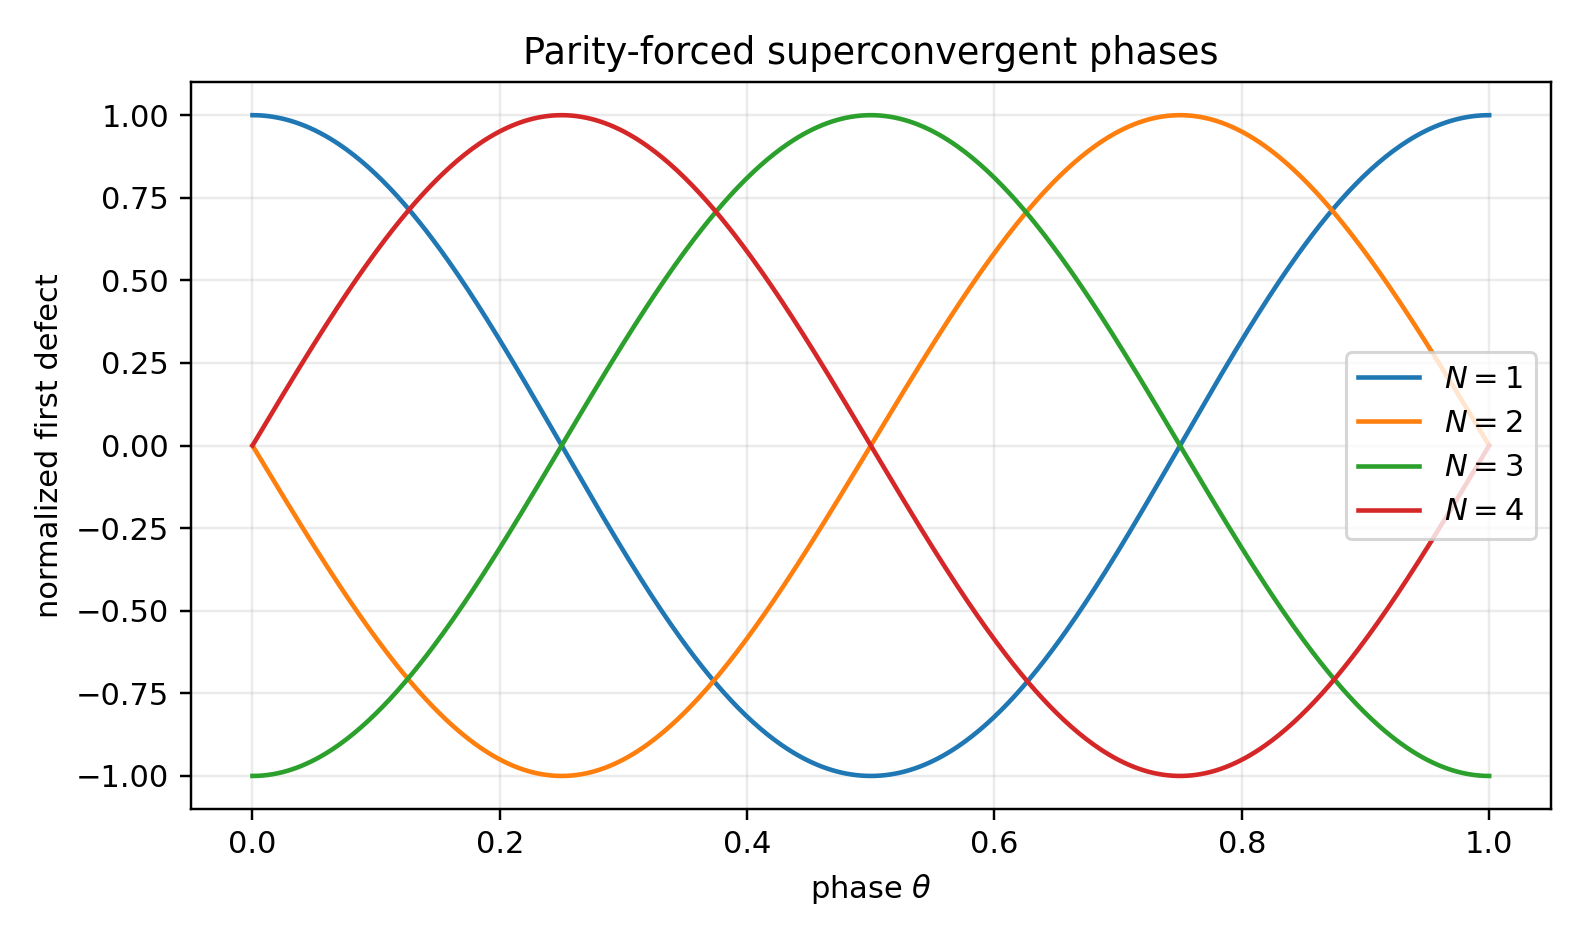
\includegraphics[width=0.88\textwidth]{assets/self-sampling/figures/defect_profiles.png}
\caption{Normalized exact first-defect profiles.  The parity-forced phases are common zeros of every odd harmonic in the corresponding sine or cosine series.}
\label{is:p3:fig:defect-profiles}
\end{figure}

\subsection{A canonical phase schedule and exact experiments}

Choose
\begin{equation}
 \theta_N=
 \begin{cases}
 0,&N\ \text{even},\\
 1/4,&N\ \text{odd}.
 \end{cases}
 \label{is:p3:eq:canonical-phase}
\end{equation}
Then $Q_{N,\theta_N}$ is positive, rational, and exact through degree $N+1$.  Its number of positive nodes is $2^{N+1}-1$ at centered levels and $2^{N+1}$ at quarter-shifted levels.

\begin{table}[H]
\centering
\caption{Exact rational checks of the canonical phase schedule.  ``Proved degree'' is the theorem above.  Each next defect is computed as an exact fraction; a decimal display is used here for legibility, while the full fractions are retained in the CSV and exact TeX table in the archive.}
\label{is:p3:tab:quadrature-exact}
% Generated by experiments.py; exact values are in the CSV
\begin{tabular}{@{}rrrrr@{}}
\toprule
$N$ & phase $\theta_N$ & positive nodes & proved degree & next defect (decimal display)\\
\midrule
0 & $0$ & 1 & 1 & $-0.11111111$\\
1 & $1/4$ & 4 & 2 & $0.011067708$\\
2 & $0$ & 7 & 3 & $0.0002806713$\\
3 & $1/4$ & 16 & 4 & $-2.189698e-6$\\
4 & $0$ & 31 & 5 & $-4.8411566e-9$\\
5 & $1/4$ & 64 & 6 & $3.0609753e-12$\\
6 & $0$ & 127 & 7 & $5.4077218e-16$\\
7 & $1/4$ & 256 & 8 & $-2.6505694e-20$\\
8 & $0$ & 511 & 9 & $-3.5647819e-25$\\
\bottomrule
\end{tabular}

\end{table}

\begin{figure}[H]
\centering
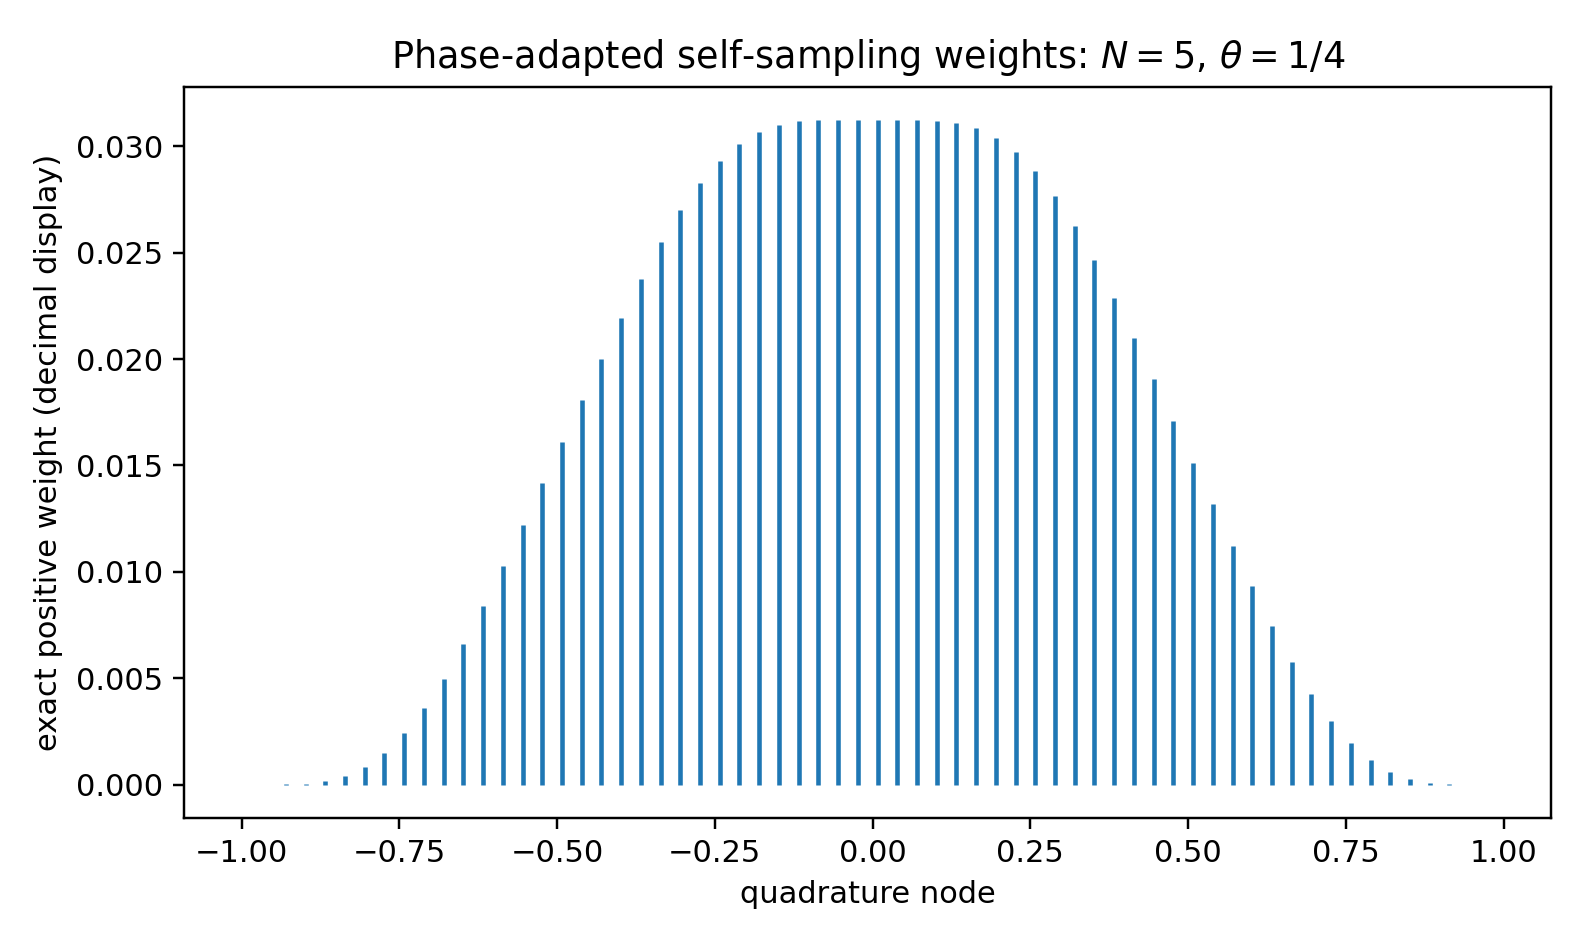
\includegraphics[width=0.88\textwidth]{assets/self-sampling/figures/quadrature_weights.png}
\caption{The positive rational weights at $N=5$, $\theta=1/4$.  The rule integrates every polynomial through degree six exactly.}
\label{is:p3:fig:quadrature-weights}
\end{figure}

The table proves by exact rational arithmetic that the canonical rule has
degree exactly $N+1$ for $0\le N\le8$.  The corresponding assertion for all
$N$, together with its experimentally observed sign refinement, is stated
once as \cref{is:p3:conj:next-defect-sign}; its exact two-layer formula is
derived in \cref{is:p3:app:next-defect}.

\section{Positive alias filters as Richardson extrapolation}
\label{is:p3:sec:positive-richardson}

\subsection{Coset rules}

For $s\ge0$ and $0\le a<2^s$, define the phase-coset rule
\begin{equation}
 Q_{N;s,a}[f]
 :=2^{-N}\sum_{k\in\IntegerNumbers}
 f\!\left(\frac{2^sk+a}{2^{N+s}}\right)
 u\!\left(\frac{2^sk+a}{2^{N+s}}\right).
 \label{is:p3:eq:coset-rule}
\end{equation}
This is simply $Q_{N,a/2^s}$, hence is positive and exact through degree $N$.

\begin{theorem}[Positive phase refinement]
\label{is:p3:thm:positive-phase-refinement}
For every $s\ge0$,
\begin{equation}
 \boxed{\displaystyle
 Q_{N+s,0}[f]
 =2^{-s}\sum_{a=0}^{2^s-1}Q_{N;s,a}[f].}
 \label{is:p3:eq:positive-phase-refinement}
\end{equation}
Thus averaging all $2^s$ positive phase classes gains exactly $s$ guaranteed degrees of polynomial exactness.
\end{theorem}

\begin{proof}
The integers $2^sk+a$, with $k\in\IntegerNumbers$ and $0\le a<2^s$, partition $\IntegerNumbers$.  Multiplying the outer factor $2^{-N}$ by $2^{-s}$ gives $2^{-(N+s)}$, exactly the fine-grid rule.
\end{proof}

For $s=1$, let
\[
 \nu_N=Q_{N,0},
 \qquad
 \rho_N=Q_{N,1/2}.
\]
Then
\begin{equation}
 \nu_{N+1}=\frac12(\nu_N+\rho_N),
 \qquad
 \boxed{\rho_N=2\nu_{N+1}-\nu_N.}
 \label{is:p3:eq:midpoint-Richardson}
\end{equation}
The right side is the familiar signed Richardson difference, yet the left side is manifestly a positive quadrature measure.  The cancellation that is hidden in scale space becomes positivity after resolution into even and odd lattice cosets.

\subsection{Uniqueness in alias space}

Suppose coefficients $c_0,\ldots,c_{2^s-1}$ combine the phase classes.  At Fourier alias $\ell$, the multiplier is
\begin{equation}
 C(\ell)=\sum_{a=0}^{2^s-1}c_a\EulerE^{2\pi\iu a\ell/2^s}.
 \label{is:p3:eq:DFT-filter}
\end{equation}
To gain all $s$ degrees, every residue class $\ell\not\equiv0\pmod{2^s}$ must be annihilated.

\begin{theorem}[Unique full residue-class filter]
\label{is:p3:thm:unique-phase-filter}
Assume
\begin{equation}
 C(0)=1,
 \qquad
 C(\ell)=0\quad(1\le\ell<2^s).
 \label{is:p3:eq:DFT-conditions}
\end{equation}
Then
\begin{equation}
 c_0=c_1=\cdots=c_{2^s-1}=2^{-s}.
 \label{is:p3:eq:unique-uniform-filter}
\end{equation}
Hence the positive average in \eqref{is:p3:eq:positive-phase-refinement} is the unique filter on all dyadic phases that cancels every nonzero residue class modulo $2^s$.
\end{theorem}

\begin{proof}
The vector $(C(0),\ldots,C(2^s-1))$ is the discrete Fourier transform of $(c_0,\ldots,c_{2^s-1})$.  Inverting the DFT of $(1,0,\ldots,0)$ gives the uniform vector.
\end{proof}

\begin{remark}[Comparison with $q$-Richardson]
The repository's geometric Lagrange/Richardson filters cancel powers of a scale parameter and generally use signed Gaussian-$q$-binomial weights.  The filter above cancels Fourier residue classes and uses equal positive weights.  The two mechanisms act in complementary variables: scale depth versus lattice phase.  Their tensor product is a natural candidate for a stable two-parameter accelerator; see \cref{is:p3:prob:hybrid-filter}.
\end{remark}

\begin{resultbox}[Third frontier bridge]
Subdividing a self-sampling rule does not merely refine a Riemann sum.  In Fourier space it applies an exact DFT projector to the alias tree.  The usual Richardson difference $2\nu_{N+1}-\nu_N$ is positive because it isolates the odd lattice coset.  This gives a rare instance in which an extrapolation operator has a hidden positive-measure realization.
\end{resultbox}

\section{Inverse-moment Rvachev--Appell polynomials}
\label{is:p3:sec:appell}

\subsection{The umbral inverse of the moment family}

The frontier volume already uses the forward moment Appell sequence
\begin{equation}
 \Pcal_n(x)=\int_{-1}^{1}(x+y)^n u(y)\Differential y,
 \qquad
 \sum_{n\ge0}\Pcal_n(x)\frac{z^n}{n!}=\EulerE^{xz}M(z).
 \label{is:p3:eq:forward-Appell}
\end{equation}
We now reverse the moment multiplier.

\begin{definition}[Sampling notation for the canonical Rvachev--Appell sequence]
\label{is:p3:def:inverse-Appell}
Set
\[
 \Acal_n(x):=A_n(x),
\]
where $A_n$ is the centered Rvachev--Appell sequence already defined in
\cref{is:p2:def:Appell-polys}.  Equivalently, its canonical generating
function reads
\begin{equation}
 \boxed{\displaystyle
 \frac{\EulerE^{xz}}{M(z)}
 =\sum_{n=0}^{\infty}\Acal_n(x)\frac{z^n}{n!}.}
 \label{is:p3:eq:inverse-Appell-gen}
\end{equation}
\end{definition}

Thus $\Acal_n$ is notation, not a second inverse-moment family.  Because
$M(0)=1$, the displayed series is well-defined formally and analytically near
$z=0$.  Its logarithm is
\begin{equation}
 xz-\sum_{r\ge1}\kappa_{2r}\frac{z^{2r}}{(2r)!}.
 \label{is:p3:eq:inverse-Appell-log}
\end{equation}

\begin{theorem}[Canonical Appell package in sampling notation]
\label{is:p3:thm:Appell-Bell}
Under the identification $\Acal_n=A_n$, the established Appell, Bell, and
operator identities take the following forms.
\begin{enumerate}
\item It is Appell and parity adapted:
\begin{equation}
 \Acal_n'(x)=n\Acal_{n-1}(x),
 \qquad
 \Acal_n(-x)=(-1)^n\Acal_n(x).
 \label{is:p3:eq:Appell-basic}
\end{equation}
\item It is a complete Bell polynomial in the Bernoulli cumulants:
\begin{equation}
 \boxed{\displaystyle
 \Acal_n(x)=Y_n(x,-\kappa_2,0,-\kappa_4,0,\ldots,-\kappa_n).}
 \label{is:p3:eq:Appell-Bell}
\end{equation}
\item It satisfies the triangular recurrence
\begin{equation}
 \Acal_{n+1}(x)
 =x\Acal_n(x)
 -\sum_{j=1}^{\Floor{(n+1)/2}}
 \binom n{2j-1}\kappa_{2j}\Acal_{n-2j+1}(x).
 \label{is:p3:eq:Appell-recurrence}
\end{equation}
\item The forward and inverse families are umbral inverses:
\begin{equation}
 M(D)\Acal_n(x)=x^n,
 \qquad
 M(D)^{-1}\Pcal_n(x)=x^n,
 \qquad D=\frac{\Differential}{\Differential x}.
 \label{is:p3:eq:umbral-inverse}
\end{equation}
\end{enumerate}
\end{theorem}

\begin{proof}
The Appell law is \eqref{is:p2:eq:Appell-derivative}, and parity follows at
once from the evenness of $M$ in the canonical generating function
\eqref{is:p2:eq:A-generating}.  Combining the canonical Bell reconstruction
\eqref{is:p2:eq:alpha-Bell} with the translation formula
\eqref{is:p2:eq:A-from-alpha} gives \eqref{is:p3:eq:Appell-Bell}; equivalently,
it is the defining complete-Bell expansion of
\eqref{is:p3:eq:inverse-Appell-log}.  The only additional displayed formula is
the convenient triangular form.  Differentiating the generating function
with respect to $z$ gives
\[
 \frac{\partial}{\partial z}\frac{\EulerE^{xz}}{M(z)}
 =\left(x-\frac{M'(z)}{M(z)}\right)\frac{\EulerE^{xz}}{M(z)},
\]
and coefficient comparison gives \eqref{is:p3:eq:Appell-recurrence}.  Finally,
the first identity in \eqref{is:p3:eq:umbral-inverse} is the canonical operator
formula \eqref{is:p2:eq:A-operator}.  The generating function
\eqref{is:p3:eq:forward-Appell} says $\Pcal_n=M(D)x^n$; applying
$M(D)^{-1}$ proves the second identity.
\end{proof}

The first polynomials are reproduced in \cref{is:p3:app:Appell-table}.  In compact notation,
\begin{align*}
 \Acal_2(x)&=x^2-\frac19,\\
 \Acal_4(x)&=x^4-\frac23x^2+\frac{31}{675},\\
 \Acal_6(x)&=x^6-\frac53x^4+\frac{31}{45}x^2-\frac{2347}{59535}.
\end{align*}
The constants are the signed complete Bell transforms of the rational cumulants; no transcendental constants remain.

\subsection{Continuous deconvolution}

\begin{theorem}[Exact deconvolution identity]
\label{is:p3:thm:Appell-deconvolution}
For every $n\ge0$ and $x\in\RealNumbers$,
\begin{equation}
 \boxed{\displaystyle
 \int_{-1}^{1}\Acal_n(x-y)u(y)\Differential y=x^n.}
 \label{is:p3:eq:Appell-deconvolution}
\end{equation}
Equivalently, the convolution operator by $u$ maps the inverse-moment Appell basis to the monomial basis.
\end{theorem}

\begin{proof}
This is the centered mean-value inversion
\eqref{is:p2:eq:mean-value-inversion}, with symmetry replacing $Y$ by $-Y$.
For completeness, the generating-function proof that will be discretized
below is as follows.  Multiply generating functions:
\begin{align*}
 \int_{-1}^{1}\frac{\EulerE^{(x-y)z}}{M(z)}u(y)\Differential y
 &=\frac{\EulerE^{xz}}{M(z)}M(-z)\\
 &=\EulerE^{xz},
\end{align*}
using the evenness $M(-z)=M(z)$.  Compare coefficients of $z^n/n!$.
\end{proof}

\begin{corollary}[Mean-zero Appell cancellations]
\label{is:p3:cor:Appell-mean-zero}
For $n\ge1$,
\begin{equation}
 \int_{-1}^{1}\Acal_n(x)u(x)\Differential x=0.
 \label{is:p3:eq:Appell-mean-zero}
\end{equation}
\end{corollary}

\begin{proof}
Set $x=0$ in \eqref{is:p3:eq:Appell-deconvolution} and use parity.
\end{proof}

\subsection{Finite lattice reproduction}

The self-sampling theorem discretizes the deconvolution identity without loss.

\begin{theorem}[Finite Rvachev--Appell translation formula]
\label{is:p3:thm:Appell-lattice-reproduction}
Let $N\ge0$, $\theta\in\RealNumbers$, and $0\le n\le N$.  Then, for every $x\in\RealNumbers$,
\begin{equation}
 \boxed{\displaystyle
 x^n=2^{-N}\sum_{k\in\IntegerNumbers}
 \Acal_n\!\left(x-\frac{k+\theta}{2^N}\right)
 u\!\left(\frac{k+\theta}{2^N}\right).}
 \label{is:p3:eq:Appell-lattice-reproduction}
\end{equation}
The sum is finite.  At a superconvergent phase from \cref{is:p3:cor:forced-superconvergence}, the identity remains valid for $n=N+1$.
\end{theorem}

\begin{proof}
For fixed $x$, the map $y\mapsto\Acal_n(x-y)$ is a polynomial of degree $n$.  Apply \cref{is:p3:thm:self-sampling} to the integral in \eqref{is:p3:eq:Appell-deconvolution}.
\end{proof}

More generally, for a polynomial $p$ define its Rvachev deconvolution
\begin{equation}
 \mathscr D_{\RvachevUp}p
 :=M(D)^{-1}p
 =\exp\!\left(-\sum_{r\ge1}\kappa_{2r}
 \frac{D^{2r}}{(2r)!}\right)p.
 \label{is:p3:eq:polynomial-deconvolution}
\end{equation}
The exponential truncates because $p$ is a polynomial.

\begin{corollary}[Polynomial reproduction by deconvolved translates]
\label{is:p3:cor:polynomial-deconvolution}
If $\deg p\le N$, then
\begin{equation}
 p(x)=2^{-N}\sum_{k\in\IntegerNumbers}
 (\mathscr D_{\RvachevUp}p)\!\left(x-\frac{k+\theta}{2^N}\right)
 u\!\left(\frac{k+\theta}{2^N}\right).
 \label{is:p3:eq:general-deconvolution-reproduction}
\end{equation}
\end{corollary}

\begin{proof}
Write $p(x)=\sum_{n=0}^{N}c_nx^n$.  The defining generating function gives
$M(D)^{-1}x^n=\Acal_n(x)$, hence
$\mathscr D_{\RvachevUp}p=\sum_{n=0}^{N}c_n\Acal_n$.  Apply
\Cref{is:p3:thm:Appell-lattice-reproduction} to each monomial and sum with
coefficients $c_n$.  Every sum is finite because $u$ is compactly supported,
so the interchange is purely finite and yields
\eqref{is:p3:eq:general-deconvolution-reproduction}.
\end{proof}

\begin{statusbox}[Lean status of Appell deconvolution and lattice reproduction]
Three source rows in this section now have exact compiled counterparts.
The centered identity \cref{is:p3:thm:Appell-deconvolution} is
\path{Fabius.integral_eval_rvachevAppellPolynomial_sub_mul_rvachev}; its
general polynomial companion is
\path{Fabius.integral_eval_rvachevDeconvolvedPolynomial_sub_mul_rvachev}.
The mean-zero corollary \cref{is:p3:cor:Appell-mean-zero} is
\path{Fabius.integral_eval_rvachevAppellPolynomial_mul_rvachev_eq_zero}, and
\cref{is:p3:cor:polynomial-deconvolution} is
\path{Fabius.normalized_tsum_shifted_rvachevDeconvolvedPolynomial_mul_rvachevUp}.
Compact support reduces the first two whole-line integrals to the displayed
interval \([-1,1]\).  The last declaration has the same nonzero natural mesh,
degree bound, arbitrary real phase, normalized physical-coordinate nodes, and
conclusion as the paper.

The full finite-lattice theorem is now formalized by an explicit two-part
family.  For arbitrary phase and $0\le n\le N$, specialize
\path{Fabius.normalized_tsum_shifted_rvachevDeconvolvedPolynomial_mul_rvachevUp}
to $M=2^N$ and $P=X^n$.  At a selected phase, including the endpoint and
midpoint pair for even $N$ and the quarter pair for odd $N$,
\path{Fabius.normalized_tsum_shifted_rvachevAppellPolynomial_mul_rvachevUp_superconvergent}
proves the same formula through $n=N+1$; the exact phase dictionary is
\path{Fabius.isRvachevSuperconvergentPhase_two_pow_iff}.  Finally,
\path{Fabius.finite_support_comb} supplies the asserted finiteness.  Thus
\cref{is:p3:thm:Appell-lattice-reproduction} is Lean-proved.  No uniqueness
or sharpness assertion about the selected phases is included in this status.
\end{statusbox}

\begin{resultbox}[Fourth frontier bridge]
The forward moment Appell family packages convolution by the up-law; the reciprocal family $\Acal_n$ packages deconvolution.  The same positive dyadic samples that integrate ordinary polynomials now reproduce ordinary monomials from translates of $\Acal_n$.  This simultaneously connects the Fourier zeros, Bernoulli cumulants, complete Bell polynomials, and finite rational Fabius values.
\end{resultbox}

\subsection{Root geometry: an exact counterexample to real-rootedness}

Numerically, the first seven polynomials have only real zeros.  Degree eight
already supplies an exact counterexample to global real-rootedness; without
exact certificates in degrees one through seven, we do not claim that it is
the first such degree.

\begin{proposition}[Exact degree-eight nonreal-zero certificate]
\label{is:p3:prop:A8-roots}
The exact polynomial
\begin{equation}
 \Acal_8(x)
 =x^8-\frac{28}{9}x^6+\frac{434}{135}x^4
 -\frac{9388}{8505}x^2+\frac{1904369}{32531625}
 \label{is:p3:eq:A8}
\end{equation}
has exactly four real zeros.  Hence its other four zeros are nonreal and form two conjugate pairs.
\end{proposition}

\begin{proof}[Computer-assisted exact proof]
Let $S_0=\Acal_8$, $S_1=S_0'$, and
$S_{j+1}=-\operatorname{rem}(S_{j-1},S_j)$ in $\RationalNumbers[x]$.
Exact Euclidean division produces nine nonzero terms, ending in the positive
constant $1904369/32531625$.  After clearing only positive rational factors,
their degrees and limiting signs are
\[
\begin{array}{c|rrrrrrrrr|c}
j&0&1&2&3&4&5&6&7&8&V\\ \hline
\deg S_j&8&7&6&5&4&3&2&1&0&\\
\Sign S_j(-\infty)&+&-&+&-&+&+&+&-&+&6\\
\Sign S_j(+\infty)&+&+&+&+&+&-&+&+&+&2
\end{array}
\]
The complete primitive integer sequence and its positive scale factors are
recorded in
\path{assets/self-sampling/appell_a8_sturm_certificate.txt}; each row may be
checked by one exact polynomial division.  Sturm's theorem therefore gives
$V(-\infty)-V(+\infty)=6-2=4$ distinct real roots.  Because the sequence
ends in a nonzero constant, $S_0$ is square-free.  Its remaining four roots
are nonreal; real coefficients pair them into two conjugate pairs.  No
floating-point root classification enters the proof.
\end{proof}

\begin{figure}[H]
\centering
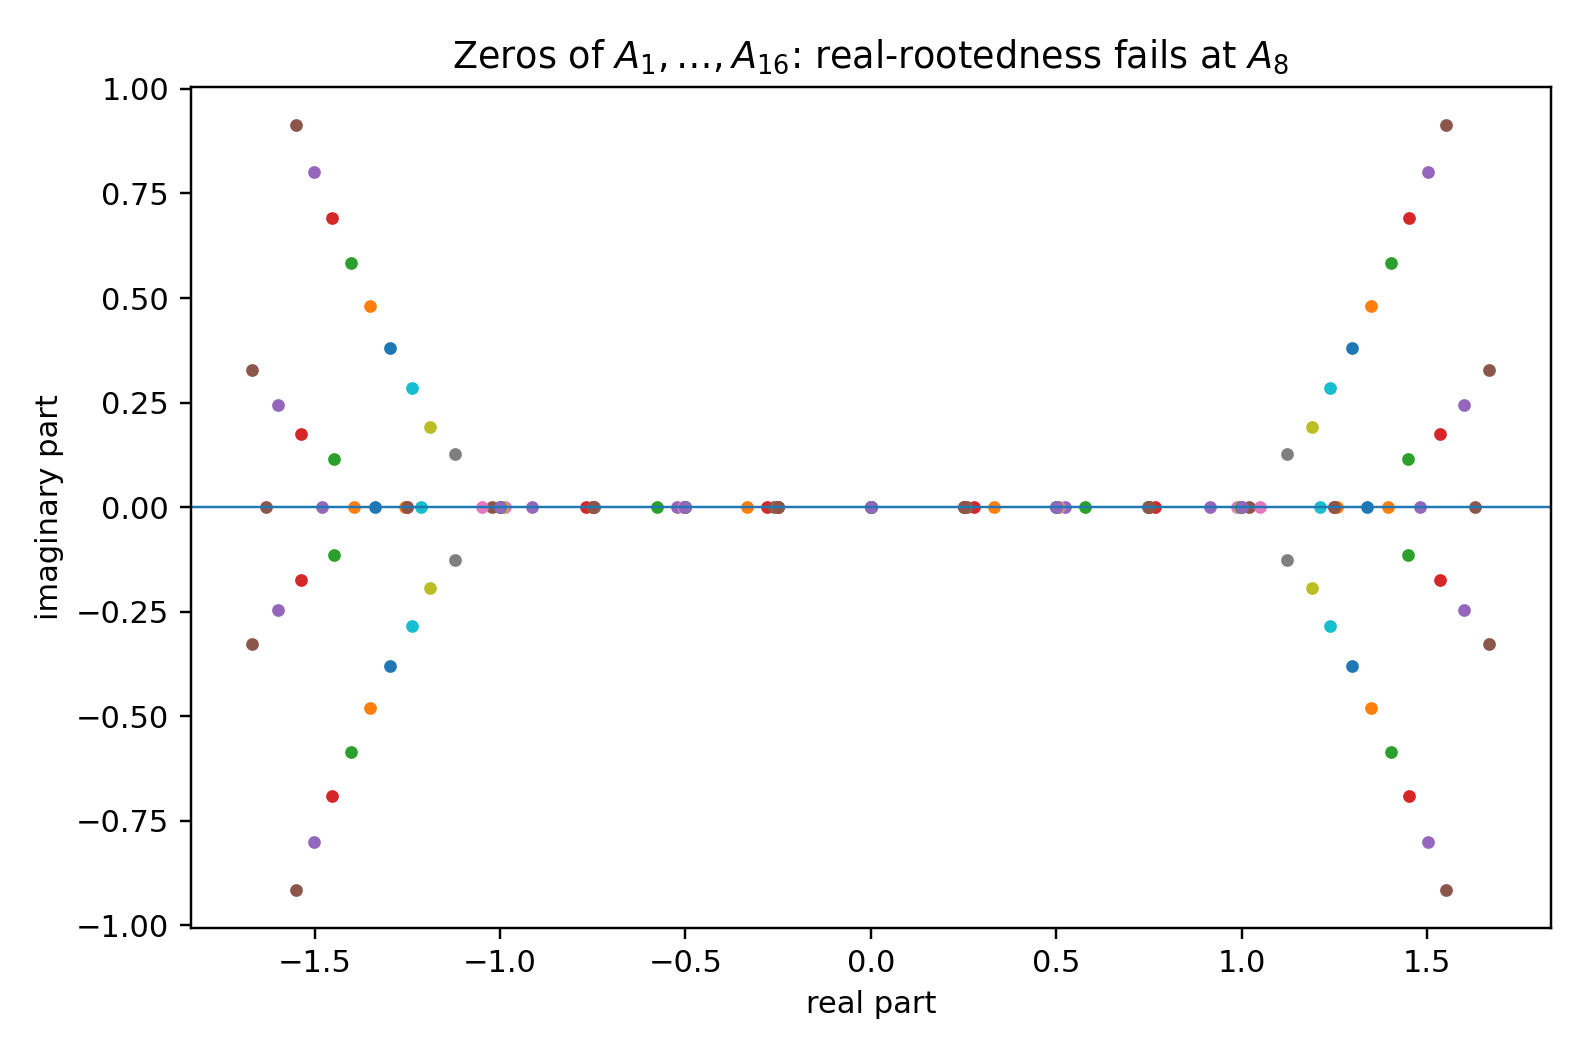
\includegraphics[width=0.86\textwidth]{assets/self-sampling/figures/appell_roots.png}
\caption{Numerical locations of the zeros of $\Acal_1,\ldots,\Acal_{16}$.
The Sturm calculation certifies the degree-eight departure from the real
axis; the apparent absence of earlier departures and the later pattern are
exploratory.}
\label{is:p3:fig:Appell-roots}
\end{figure}

The computed nonreal-root counts through degree $30$ are
\begin{center}
\begin{tabular}{@{}lrrrrrr@{}}
\toprule
Degree range & $1$--$7$ & $8$--$12$ & $13$--$17$ & $18$--$22$ & $23$--$28$ & $29$--$30$\\
\midrule
Nonreal roots & $0$ & $4$ & $8$ & $12$ & $16$ & $20$\\
\bottomrule
\end{tabular}
\end{center}
This staircase is not asserted as a theorem; it motivates \cref{is:p3:conj:Appell-root-staircase}.

\section{Transport through the inverse Fabius function}
\label{is:p3:sec:inverse-transport}

The centered quantile $q(t)=2F^{-1}(t)-1$ pushes Lebesgue measure on $[0,1]$ to the up-law.  Therefore
\begin{equation}
 \int_0^1g(q(t))\Differential t=\int_{-1}^{1}g(x)u(x)\Differential x
 \label{is:p3:eq:quantile-transport}
\end{equation}
for every bounded Borel function $g$.

\begin{theorem}[Rational inverse-Fabius quadrature]
\label{is:p3:thm:inverse-Fabius-quadrature}
Let $\theta=a/2^s$ and retain the dyadic nodes $x_k=n_k/2^D$ and weights $w_k$ from \cref{is:p3:cor:rational-rules}.  Define
\begin{equation}
 t_k=F\!\left(\frac{1+x_k}{2}\right)\in\RationalNumbers.
 \label{is:p3:eq:inverse-Fabius-nodes}
\end{equation}
Then $q(t_k)=x_k$, and for every polynomial $p$ with $\deg p\le N$,
\begin{equation}
 \boxed{\displaystyle
 \int_0^1p\bigl(2F^{-1}(t)-1\bigr)\Differential t
 =\sum_k w_k\,p\bigl(2F^{-1}(t_k)-1\bigr)
 =\sum_k w_kp(x_k).}
 \label{is:p3:eq:inverse-Fabius-quadrature}
\end{equation}
At a phase-superconvergent level the exactness extends to $\deg p\le N+1$.
\end{theorem}

\begin{proof}
Equation \eqref{is:p3:eq:centered-CDF} implies $q(t_k)=x_k$.  Apply \eqref{is:p3:eq:quantile-transport} and then \cref{is:p3:thm:self-sampling}.  Rationality follows because both $(1+x_k)/2$ and the weight arguments are dyadic.
\end{proof}

\begin{remark}[A nonlinear exactness space]
The rule in \eqref{is:p3:eq:inverse-Fabius-quadrature} is not claimed to integrate all ordinary polynomials in $t$.  It integrates exactly the non-elementary space
\begin{equation}
 \mathcal V_N
 =\SpanOperator\{1,q(t),q(t)^2,\ldots,q(t)^N\},
 \qquad q(t)=2F^{-1}(t)-1,
 \label{is:p3:eq:inverse-exactness-space}
\end{equation}
using rational nodes $t_k$, rational weights $w_k$, and no numerical inversion.  This is an exact finite interface between the inverse Fabius function and dyadic arithmetic.
\end{remark}

\subsection{Endpoint nodes and the Lambert coordinate}

For centered rules, the smallest nonzero endpoint distance is $2^{-N}$ and the corresponding extreme weights are
\begin{equation}
 2^{-N}F(2^{-N}).
 \label{is:p3:eq:centered-extreme-weight}
\end{equation}
For quarter-shifted rules, the leftmost distance is $2^{-N-2}$, so one extreme weight is
\begin{equation}
 2^{-N}F(2^{-N-2}).
 \label{is:p3:eq:quarter-extreme-weight}
\end{equation}
The corpus's sharp endpoint theory expresses $F(x)$ through the exact lower-Lambert coordinate
\begin{equation}
 \lambda(x)=-\frac1{\log2}W_{-1}(-x\log2),
 \qquad x=\lambda2^{-\lambda},
 \label{is:p3:eq:Lambert-coordinate}
\end{equation}
with a nonconstant periodic correction in the dyadic phase of $\lambda$.  Thus the new quadrature rules supply exact rational global moment constraints whose smallest weights lie precisely in the Lambert boundary layer.  Turning these constraints into identities for the endpoint periodic factor is an open program formulated in \cref{is:p3:prob:Lambert-sum-rules}.

\section{Finite Gaussian-\texorpdfstring{$q$}{q}-binomial identities forced by quadrature}
\label{is:p3:sec:qbinomial}

\subsection{The exact dyadic evaluator}

Let
\begin{equation}
 (q;q)_n=\prod_{j=1}^{n}(1-q^j),
 \qquad
 \GaussianBinomial{n}{k}{q}=\frac{(q;q)_n}{(q;q)_k(q;q)_{n-k}}.
 \label{is:p3:eq:q-notation-report}
\end{equation}
For integers $m,n\ge0$ and $c\in\RationalNumbers$, define
\begin{equation}
\begin{aligned}
 \mathfrak Q_n(m;c)
 :={}&\frac{1}{2^{n^2}(1/2;1/2)_n}
 \sum_{j=0}^{n}
 \frac{\GaussianBinomial{n}{j}{1/2}}
      {2^{j(j-1)}(n+j)!}\\
 &\qquad\times
 \sum_{r=0}^{m2^j-1}\eps_r
 \bigl(r-m2^j+c\bigr)^{n+j}.
 \label{is:p3:eq:Qfrak-def}
\end{aligned}
\end{equation}
The established arbitrary-numerator theorem states
\begin{equation}
 \mathfrak Q_n(m;c)=F(m/2^n)
 \qquad(0\le m\le2^n),
 \label{is:p3:eq:Qfrak-F}
\end{equation}
and the right side of \eqref{is:p3:eq:Qfrak-def} is independent of $c$.  Its Gaussian coefficients arise from Lagrange interpolation on a geometric grid.

\subsection{A \texorpdfstring{$q$}{q}-binomial--Thue--Morse--Bell identity}

\begin{theorem}[Finite arithmetic moment identity]
\label{is:p3:thm:qbinomial-moment-identity}
Let $\theta=a/2^s$, $D=N+s$, $n_k=2^sk+a$, and $b_k=2^D-\AbsoluteValue{n_k}$.  For every $0\le r\le N$ and every $c\in\RationalNumbers$,
\begin{equation}
 \boxed{\displaystyle
 \mu_r
 =2^{-N-Dr}
 \sum_{\AbsoluteValue{n_k}<2^D}
 n_k^r\,\mathfrak Q_D(b_k;c).}
 \label{is:p3:eq:qbinomial-moment-identity}
\end{equation}
At the superconvergent phases of \cref{is:p3:cor:forced-superconvergence}, the identity also holds for $r=N+1$.  Therefore the finite Gaussian-$q$-binomial--Thue--Morse sum on the right equals
\begin{equation}
 Y_r(0,\kappa_2,0,\kappa_4,\ldots,\kappa_r),
 \label{is:p3:eq:qbinomial-Bell-right}
\end{equation}
where the cumulants are the Bernoulli rationals in \eqref{is:p3:eq:cumulants}.
\end{theorem}

\begin{proof}
At node $x_k=n_k/2^D$, \eqref{is:p3:eq:F-up-relation} and \eqref{is:p3:eq:Qfrak-F} give
\[
 u(x_k)=F(b_k/2^D)=\mathfrak Q_D(b_k;c).
\]
Substitute this into \eqref{is:p3:eq:self-sampling-main}, then use \eqref{is:p3:eq:moment-Bell}.
\end{proof}

\begin{remark}[Why this identity is structurally new]
Each ingredient existed separately: the $q$-binomial evaluator, the Bell moment formula, and the zero multiplicities.  The self-sampling theorem forces them into a single positive finite identity.  The common translation $c$ disappears after a double finite summation, giving a family of nontrivial translation-invariance identities among Thue--Morse power sums.
\end{remark}

\begin{corollary}[Finite Appell cancellation in $q$-arithmetic]
\label{is:p3:cor:q-Appell-cancellation}
For $1\le n\le N$,
\begin{equation}
 \sum_{\AbsoluteValue{n_k}<2^D}
 \Acal_n\!\left(-\frac{n_k}{2^D}\right)
 \mathfrak Q_D(b_k;c)=0.
 \label{is:p3:eq:q-Appell-cancellation}
\end{equation}
After inserting \eqref{is:p3:eq:Qfrak-def}, this is a finite identity containing Gaussian $q$-binomial coefficients, Thue--Morse signs, Bernoulli cumulants, and complete Bell polynomials.
\end{corollary}

\begin{proof}
Set $x=0$ in \eqref{is:p3:eq:Appell-lattice-reproduction} and clear the common factor $2^{-N}$.
\end{proof}

\section{Base-\texorpdfstring{$b$}{b} and multidimensional extensions}
\label{is:p3:sec:extensions}

\subsection{Integer dilation bases}

Let $b\ge2$ be an integer and define
\begin{equation}
 \Phi_b(\xi)=\prod_{j=0}^{\infty}
 \SincPi\!\left(\frac{\xi}{b^j}\right).
 \label{is:p3:eq:Phi-b}
\end{equation}

\begin{proposition}[Construction and regularity of the base-$b$ density]
\label{is:p3:prop:base-b-density}
Let $(U_j)_{j\ge0}$ be independent, with $U_j$ uniform on
\[
 I_j=\left[-\frac1{2b^j},\frac1{2b^j}\right].
\]
Then the series $S_b=\sum_{j\ge0}U_j$ converges absolutely.  Its law has a
nonnegative density $u_b\in C_c^\infty(\RealNumbers)$ satisfying
\begin{equation}
 \FourierTwoPi{u_b}(\xi)=\Phi_b(\xi),
 \qquad
 \int_{\RealNumbers}u_b(x)\Differential x=1,
 \qquad
 \SupportOperator(u_b)=
 \left[-\frac{b}{2(b-1)},\frac{b}{2(b-1)}\right].
 \label{is:p3:eq:base-b-density-properties}
\end{equation}
Thus $u_b$ is precisely the infinite convolution of the centered uniform
density factors.
\end{proposition}

\begin{proof}
The deterministic estimate
\[
 \sum_{j\ge0}\AbsoluteValue{U_j}
 \le\frac12\sum_{j\ge0}b^{-j}=\frac{b}{2(b-1)}
\]
proves absolute convergence.  The $j$th uniform law has Fourier transform
$\SincPi(\xi/b^j)$, so independence and convergence of the partial sums give
$\Expectation\EulerE^{-2\pi\iu\xi S_b}=\Phi_b(\xi)$.

It remains to justify that this probability law is smooth rather than merely
a compactly supported measure.  The elementary estimate
\[
 \AbsoluteValue{\SincPi t}\le
 \min\left(1,\frac1{\pi\AbsoluteValue t}\right)
\]
shows, by retaining any fixed number $K$ of factors in
\eqref{is:p3:eq:Phi-b}, that
\[
 \AbsoluteValue{\Phi_b(\xi)}\le C_K(1+\AbsoluteValue\xi)^{-K}
 \qquad(\xi\in\RealNumbers)
\]
for some constant $C_K$.  Hence $\xi^r\Phi_b(\xi)$ is integrable for every
$r\ge0$.  Fourier inversion therefore supplies a $C^r$ density for every
$r$, and differentiating under the inverse-transform integral identifies all
of its derivatives.  Thus $u_b\in C^\infty$.  Since it represents a
probability law, it is nonnegative and has integral one.

For the exact support, equip $\prod_{j\ge0}I_j$ with the product measure.  It
has full support, and the summation map is continuous because the defining
series converges uniformly.  Its image is the interval
\[
 \sum_{j\ge0}I_j=
 \left[-\frac12\sum_{j\ge0}b^{-j},
        \frac12\sum_{j\ge0}b^{-j}\right]
 =\left[-\frac{b}{2(b-1)},\frac{b}{2(b-1)}\right].
\]
(For example, every point in this interval is obtained by choosing all
coordinates in the same fixed proportion of their respective endpoints.)
The continuous image of this full-support product measure consequently has
exactly that interval as its support.  This proves
\eqref{is:p3:eq:base-b-density-properties}.
\end{proof}

If $m\ne0$ is an integer, then
\begin{equation}
 \OrderOperator_{\xi=m}\Phi_b=1+\nu_b(m),
 \label{is:p3:eq:b-multiplicity}
\end{equation}
where $\nu_b(m)$ is the largest $a$ such that $b^a\mid m$.
Indeed, precisely the factors with $0\le j\le\nu_b(m)$ vanish at $m$; each
has a simple zero there, and every later factor is nonzero.

\begin{theorem}[Base-$b$ self-sampling]
\label{is:p3:thm:base-b}
For every $N\ge0$, phase $\theta$, and polynomial $p$ of degree at most $N$,
\begin{equation}
 \int p(x)u_b(x)\Differential x
 =b^{-N}\sum_{k\in\IntegerNumbers}
 p\!\left(\frac{k+\theta}{b^N}\right)
 u_b\!\left(\frac{k+\theta}{b^N}\right).
 \label{is:p3:eq:base-b-self-sampling}
\end{equation}
Moreover, averaging the $b^s$ phases $a/b^s$ gives the level-$N+s$ rule and is
the unique normalized full DFT filter: among coefficient vectors $(c_a)$ with
$\sum_a c_a=1$, it is the only one annihilating every nonzero residue modulo
$b^s$.
\end{theorem}

\begin{proof}
By \cref{is:p3:prop:base-b-density}, the functions
$x^ru_b(x)$ are smooth and compactly supported, so Poisson summation applies.
For $0\le r\le N$, its nonzero alias at $b^N\ell$ is a constant multiple of
$\Phi_b^{(r)}(b^N\ell)$.  Equation \eqref{is:p3:eq:b-multiplicity} gives
\[
 \OrderOperator_{\xi=b^N\ell}\Phi_b
 =N+1+\nu_b(\ell)>r,
\]
so every such alias vanishes.  The zero alias is the $r$th moment.  This proves
\eqref{is:p3:eq:base-b-self-sampling} for monomials and hence for all stated
polynomials.

For the phase refinement, average the rules with phases $a/b^s$.  Writing
$r=b^sk+a$ identifies their nodes bijectively with $r/b^{N+s}$, and the
averaged coefficient is $b^{-(N+s)}$; the result is exactly the level-$N+s$
rule.  Finally, normalized weights $c_a$ with $\sum_a c_a=1$ annihilate every
nonzero residue precisely when their $b^s$-point discrete Fourier transform is
$(1,0,\ldots,0)$.  Fourier
inversion gives $c_a=b^{-s}$ for every $a$, proving uniqueness.
\end{proof}

The binary case is distinguished arithmetically because half-integer spectral signs reduce to the classical Thue--Morse sequence and dyadic Fabius values are rational.  For general $b$, the same analytic framework suggests generalized digital sign sequences and $q=b^{-1}$ arithmetic.

\subsection{Tensor-product cubature}

Let
\begin{equation}
 U_d(x_1,\ldots,x_d)=\prod_{j=1}^{d}u(x_j).
 \label{is:p3:eq:tensor-density}
\end{equation}
Tensoring \cref{is:p3:thm:self-sampling} gives a positive cubature rule.

\begin{corollary}[Positive tensor cubature]
\label{is:p3:cor:tensor-cubature}
For a polynomial $p$ whose degree in each coordinate is at most $N$,
\begin{equation}
 \int_{[-1,1]^d}p(\bm x)U_d(\bm x)\Differential\bm x
 =2^{-Nd}\sum_{\bm k\in\IntegerNumbers^d}
 p\!\left(\frac{\bm k+\bm\theta}{2^N}\right)
 U_d\!\left(\frac{\bm k+\bm\theta}{2^N}\right).
 \label{is:p3:eq:tensor-cubature}
\end{equation}
The sum is finite and positive.  Coordinatewise phase superconvergence raises the exactness by one in every selected coordinate.
\end{corollary}

\begin{proof}
It is enough by linearity to take
$p(\bm x)=\prod_{j=1}^{d}x_j^{r_j}$ with $0\le r_j\le N$.  Fubini's theorem
factors the integral into $d$ one-dimensional moments.  Apply
\Cref{is:p3:thm:self-sampling} to each factor and multiply the resulting
finite sums; their Cartesian product is exactly
\eqref{is:p3:eq:tensor-cubature}.  Compact support makes the sum finite, and
every weight is nonnegative because $u\ge0$.  If a chosen coordinate phase
satisfies the cancellation condition of
\Cref{is:p3:cor:forced-superconvergence}, the same argument admits
$r_j=N+1$ in that coordinate; applying this independently proves the final
coordinatewise assertion.
\end{proof}

The node count grows exponentially with $d$, so sparse-grid combinations and hyperbolic-cross alias filters are a natural next step; see \cref{is:p3:prob:sparse-grid}.

% Source fragment: Inverse and sampling frontiers; prefix is.
\section{Conjectures and frontier research program}
\label{is:p3:sec:frontier}

\subsection{The next alias layer}

\begin{conjecture}[Exact phase-adapted precision and sign]
\label{is:p3:conj:next-defect-sign}
Let $\theta_N$ be the canonical phase in \eqref{is:p3:eq:canonical-phase}.  Then
\begin{equation}
 E_{N,N+2}(\theta_N)\ne0
 \qquad(N\ge0).
 \label{is:p3:eq:next-defect-nonzero}
\end{equation}
Moreover, for $N\ge1$, the experimental sign law is
\begin{equation}
 \Sign E_{N,N+2}(\theta_N)
 =(-1)^{\Floor{(N-1)/2}}.
 \label{is:p3:eq:next-defect-sign-conj}
\end{equation}
\end{conjecture}

The exact two-layer formula is given in \cref{is:p3:app:next-defect}.  A proof should combine:
\begin{enumerate}
\item the odd-alias contribution with one Bell correction $\gamma_1$;
\item the twice-odd contribution with its leading zero jet;
\item the parity-specific phase factors;
\item a first-frequency dominance estimate sharp enough to control the logarithmic derivative $\PhiCyc'/\PhiCyc$ at half-integers.
\end{enumerate}
A successful argument would determine the exact degree of every positive phase-adapted rule.

\begin{problem}[All higher phase gains]
\label{is:p3:prob:higher-phase-gains}
For fixed excess $s\ge2$, classify all phases $\theta$ for which
\[
 E_{N,N+1}(\theta)=\cdots=E_{N,N+s}(\theta)=0.
\]
The valuation filtration makes this a finite hierarchy of trigonometric equations built from alias layers $0,\ldots,s-1$.  Determine whether any single positive phase can gain more than one degree for infinitely many $N$.
\end{problem}

\subsection{Optimal phase and scale filters}

\begin{problem}[Hybrid DFT--Gaussian-$q$ filter]
\label{is:p3:prob:hybrid-filter}
Combine the positive DFT projector in \eqref{is:p3:eq:positive-phase-refinement} with the repository's geometric Gaussian-$q$-binomial Richardson filters in the scale variable.  For a prescribed exactness order, minimize:
\begin{enumerate}
\item total variation of the combined coefficients;
\item number of distinct dyadic Fabius evaluations;
\item largest denominator of an exact rational coefficient;
\item sensitivity near the flat endpoints.
\end{enumerate}
A two-stage construction may first remove low $2$-adic alias classes by positive phase averaging and then remove the remaining scale modes by a short signed $q$-Richardson filter.
\end{problem}

\begin{problem}[Sparse positive phase design]
\label{is:p3:prob:sparse-positive-phase}
Fix $s\ge2$ and $1\le q<2^s$.  Among probability vectors
$c=(c_0,\ldots,c_{2^s-1})$ with at most $q$ nonzero entries, determine
\[
 \min_c\;\max_{1\le r<2^s}
 \left|\sum_{a=0}^{2^s-1}c_a
       \EulerE^{2\pi\ImaginaryUnit ar/2^s}\right|,
\]
classify the minimizers up to cyclic symmetry, and, among tied minimizers,
minimize $\sum_ac_a^2$.  Determine how the optimal leakage controls the
worst first surviving alias of the associated positive sampling rule.
\end{problem}

The former ``positive extremality'' conjecture imposed all exact DFT
annihilation equations.  By \Cref{is:p3:thm:unique-phase-filter} those
equations admit only the uniform vector, so optimization over that singleton
was vacuous.  The support constraint above creates a genuine tradeoff between
positivity, sparsity, and alias suppression.

\subsection{Denominators and arithmetic geometry}

\begin{problem}[Exact valuations of self-sampling weights]
\label{is:p3:prob:weight-valuations}
For dyadic $\theta=a/2^s$, determine the exact prime valuations of
\[
 w_{N,\theta,k}=2^{-N}F\!\left(1-\frac{\AbsoluteValue{2^sk+a}}{2^{N+s}}\right)
\]
in lowest terms.  Natural targets are:
\begin{enumerate}
\item exact $2$-adic valuations of the extreme weights;
\item odd-prime divisibility controlled by Mersenne factors $2^{2j}-1$;
\item the least common denominator of the complete rule;
\item cancellation in the rational next defect $E_{N,N+2}(\theta_N)$.
\end{enumerate}
The q-binomial identity \eqref{is:p3:eq:qbinomial-moment-identity} supplies a second route to the same valuations and may reveal cancellations invisible in the moment formula.
\end{problem}

The former ``primitive normalized phase rules'' conjecture is also retired.
If $L$ is defined to be the \emph{least} common denominator of a rational
weight vector, then the integers $Lw_k$ automatically have greatest common
divisor one: their gcd divides $L$ because $\sum_kLw_k=L$, and a larger gcd
would produce a smaller common denominator.  The nontrivial arithmetic
question is therefore the exact value and prime factorization of $L$, already
posed in \Cref{is:p3:prob:weight-valuations}.

\subsection{Rvachev--Appell zero geometry}

\begin{conjecture}[Unbounded nonreal root count]
\label{is:p3:conj:Appell-root-staircase}
The number of nonreal zeros of $\Acal_n$ tends to infinity with $n$.
\end{conjecture}

This statement deliberately does not extrapolate the short numerical
staircase.  A stronger, separately testable target is weak convergence of the
empirical measures
\[
 \nu_n:=\frac1n\sum_{\Acal_n(z)=0}\delta_{2\pi z/n}
\]
(zeros counted with multiplicity) to a probability measure with compact
support.  Identifying such a measure and its support belongs to the spectral
problem below; measures converge to measures, not to compact sets.

\begin{problem}[A spectral asymptotic for $\Acal_n$]
\label{is:p3:prob:Appell-spectral-asymptotic}
Use residues of $\EulerE^{xz}/M(z)$ to derive an expansion for $\Acal_n(x)/n!$ that is uniform in the zero-scaling regime.  Determine:
\begin{enumerate}
\item the first curve on which the contributions from $\pm2\pi\iu$ balance;
\item how the next dyadic poles perturb that curve;
\item whether the observed root-count plateaus have an exact spectral explanation;
\item whether a Jensen-polynomial or multiplier-sequence normalization restores real-rootedness.
\end{enumerate}
\end{problem}

\subsection{Lambert endpoint sum rules}

\begin{problem}[Exact quadrature constraints on the periodic endpoint factor]
\label{is:p3:prob:Lambert-sum-rules}
Insert the repository's all-orders endpoint expansion for $F(x)$, written in the lower-Lambert coordinate \eqref{is:p3:eq:Lambert-coordinate}, into the exact identities \eqref{is:p3:eq:centered-moment-F} and \eqref{is:p3:eq:qbinomial-moment-identity}.  After separating the bulk from a shrinking endpoint boundary layer, derive explicit linear or nonlinear sum rules for the periodic coefficient functions.
\end{problem}

The principal difficulty is uniformity: the number of dyadic samples grows with $N$, while the Lambert expansion is strongest only near the endpoints.  A viable strategy is to choose a cutoff $j\le J(N)$, use the endpoint transseries on that range, and control the remaining samples by smooth quadrature estimates.  Exactness of the full moment identity should force cancellation between the two endpoint layers and the bulk.

\begin{problem}[Uniform endpoint/alias matching for extreme quantile nodes]
\label{is:p3:prob:quantile-endpoint-alias}
For the inverse-Fabius quadrature in
\eqref{is:p3:eq:inverse-Fabius-quadrature}, choose an explicit cutoff
$J(N)\to\infty$ with $J(N)=o(2^N)$.  Derive a lower-Lambert expansion,
uniform for the extreme indices $0\le k\le J(N)$ and their reflected partners,
with a stated remainder after each retained inverse-phase order.  Then define
an explicit two-level combination of the phases in
\eqref{is:p3:eq:canonical-phase} and determine whether its normalized
endpoint contribution cancels through one additional inverse-phase order;
bound the complementary bulk uniformly so that the resulting assertion is a
theorem about the complete quadrature error.
\end{problem}

The earlier phase-locking wording did not specify the extreme-index schedule,
the two-level coefficients, the normalization, or the meaning of one
inverse-Lambert order.  Those data are made explicit requirements here rather
than hidden inside an unfalsifiable conjecture.

\subsection{Digital generalizations and higher dimensions}

\begin{problem}[Base-$b$ spectral signs]
\label{is:p3:prob:base-b-signs}
For the product \eqref{is:p3:eq:Phi-b}, determine the sign and phase of $\Phi_b((bk+r)/b)$ on each nonzero residue class $r$.  Identify the resulting automatic sequence and its analogues of Prouhet cancellation, Mahler equations, and $q$-binomial arithmetic.
\end{problem}

\begin{problem}[Sparse-grid Rvachev cubature]
\label{is:p3:prob:sparse-grid}
Construct Smolyak or hyperbolic-cross combinations of the tensor rules \eqref{is:p3:eq:tensor-cubature} that preserve as much positivity as possible.  The alias description suggests indexing components by $2$-adic valuation vectors rather than by total scale alone.  Determine optimal node counts for coordinatewise or total-degree exactness.
\end{problem}

\begin{problem}[Nonproduct Rvachev laws]
\label{is:p3:prob:nonproduct-laws}
Replace the tensor product by compactly supported refinable densities associated with a dilation matrix.  Characterize when Fourier zero multiplicities on the dual lattice make the density's own samples into a positive polynomial cubature rule.
\end{problem}

% Source fragment: Inverse and sampling frontiers; prefix is.
\section{First inverse-moment Appell polynomials}
\label{is:p3:app:Appell-table}

For compactness the generated table writes $A_n$ in place of $\Acal_n$.
% Generated exactly by experiments.py
\begin{align*}
A_{0}(x)&=1\\
A_{1}(x)&=x\\
A_{2}(x)&=x^{2} - \frac{1}{9}\\
A_{3}(x)&=x^{3} - \frac{x}{3}\\
A_{4}(x)&=x^{4} - \frac{2 x^{2}}{3} + \frac{31}{675}\\
A_{5}(x)&=x^{5} - \frac{10 x^{3}}{9} + \frac{31 x}{135}\\
A_{6}(x)&=x^{6} - \frac{5 x^{4}}{3} + \frac{31 x^{2}}{45} - \frac{2347}{59535}\\
A_{7}(x)&=x^{7} - \frac{7 x^{5}}{3} + \frac{217 x^{3}}{135} - \frac{2347 x}{8505}\\
A_{8}(x)&=x^{8} - \frac{28 x^{6}}{9} + \frac{434 x^{4}}{135} - \frac{9388 x^{2}}{8505} + \frac{1904369}{32531625}\\
A_{9}(x)&=x^{9} - 4 x^{7} + \frac{434 x^{5}}{75} - \frac{9388 x^{3}}{2835} + \frac{1904369 x}{3614625}\\
A_{10}(x)&=x^{10} - 5 x^{8} + \frac{434 x^{6}}{45} - \frac{4694 x^{4}}{567} + \frac{1904369 x^{2}}{722925} - \frac{3309760579}{24405225075}
\end{align*}


\section{Exact two-layer formula for the next defect}
\label{is:p3:app:next-defect}

Put $R=N+2$.  The valuation filtration \eqref{is:p3:eq:valuation-filtration} contains only $a=0$ and $a=1$.  For odd $q$, define
\begin{align}
 m_0&=2^Nq,&d_0&=N+1,\\
 m_1&=2^{N+1}q,&d_1&=N+2=R.
\end{align}
Then \cref{is:p3:cor:Bell-zero-jets} gives
\begin{align}
 \PhiCyc^{(R)}(m_0)
 &=-\frac{R!\PhiCyc(q/2)}{m_0^{N+1}}\gamma_1(m_0),
 \label{is:p3:eq:next-defect-layer0}\\
 \PhiCyc^{(R)}(m_1)
 &=-\frac{R!\PhiCyc(q/2)}{m_1^R}.
 \label{is:p3:eq:next-defect-layer1}
\end{align}
Consequently
\begin{equation}
\boxed{
\begin{aligned}
 E_{N,N+2}(\theta)
 =-\frac{R!}{(-2\pi\iu)^R}
 \sum_{\substack{q\in\IntegerNumbers\setminus\{0\}\\q\ \mathrm{odd}}}
 \PhiCyc(q/2)\Bigg[&
 \frac{\gamma_1(2^Nq)}{(2^Nq)^{N+1}}
 \EulerE^{2\pi\iu q\theta}\\
 &+\frac{1}{(2^{N+1}q)^R}
 \EulerE^{4\pi\iu q\theta}\Bigg].
\end{aligned}}
\label{is:p3:eq:next-defect-exact}
\end{equation}
Here
\begin{equation}
 \gamma_1(2^Nq)
 =-\frac{N+1}{2^Nq}
 +2^{-N-1}\frac{\PhiCyc'(q/2)}{\PhiCyc(q/2)}.
 \label{is:p3:eq:next-defect-gamma1}
\end{equation}
This formula is the proposed starting point for \cref{is:p3:conj:next-defect-sign}.  It isolates exactly what is new beyond the first defect: a half-integer logarithmic derivative and one newly activated $2$-adic alias layer.
